% =========================================================
\section{TEF-RAG Method}
\label{sec:method}
% =========================================================

Figure~\ref{fig:tef_overview} presents the overall TEF-RAG pipeline. The method consists of four connected stages: legal-candidate retrieval, learned evidence-pair proposal, query-conditioned relation graph construction, and nonlinear set ranking. The first two stages control candidate size, the relation graph represents process structure among evidence records, and the final ranker directly compares the overall utility of candidate evidence sets.

\begin{figure*}[t]
    \centering
    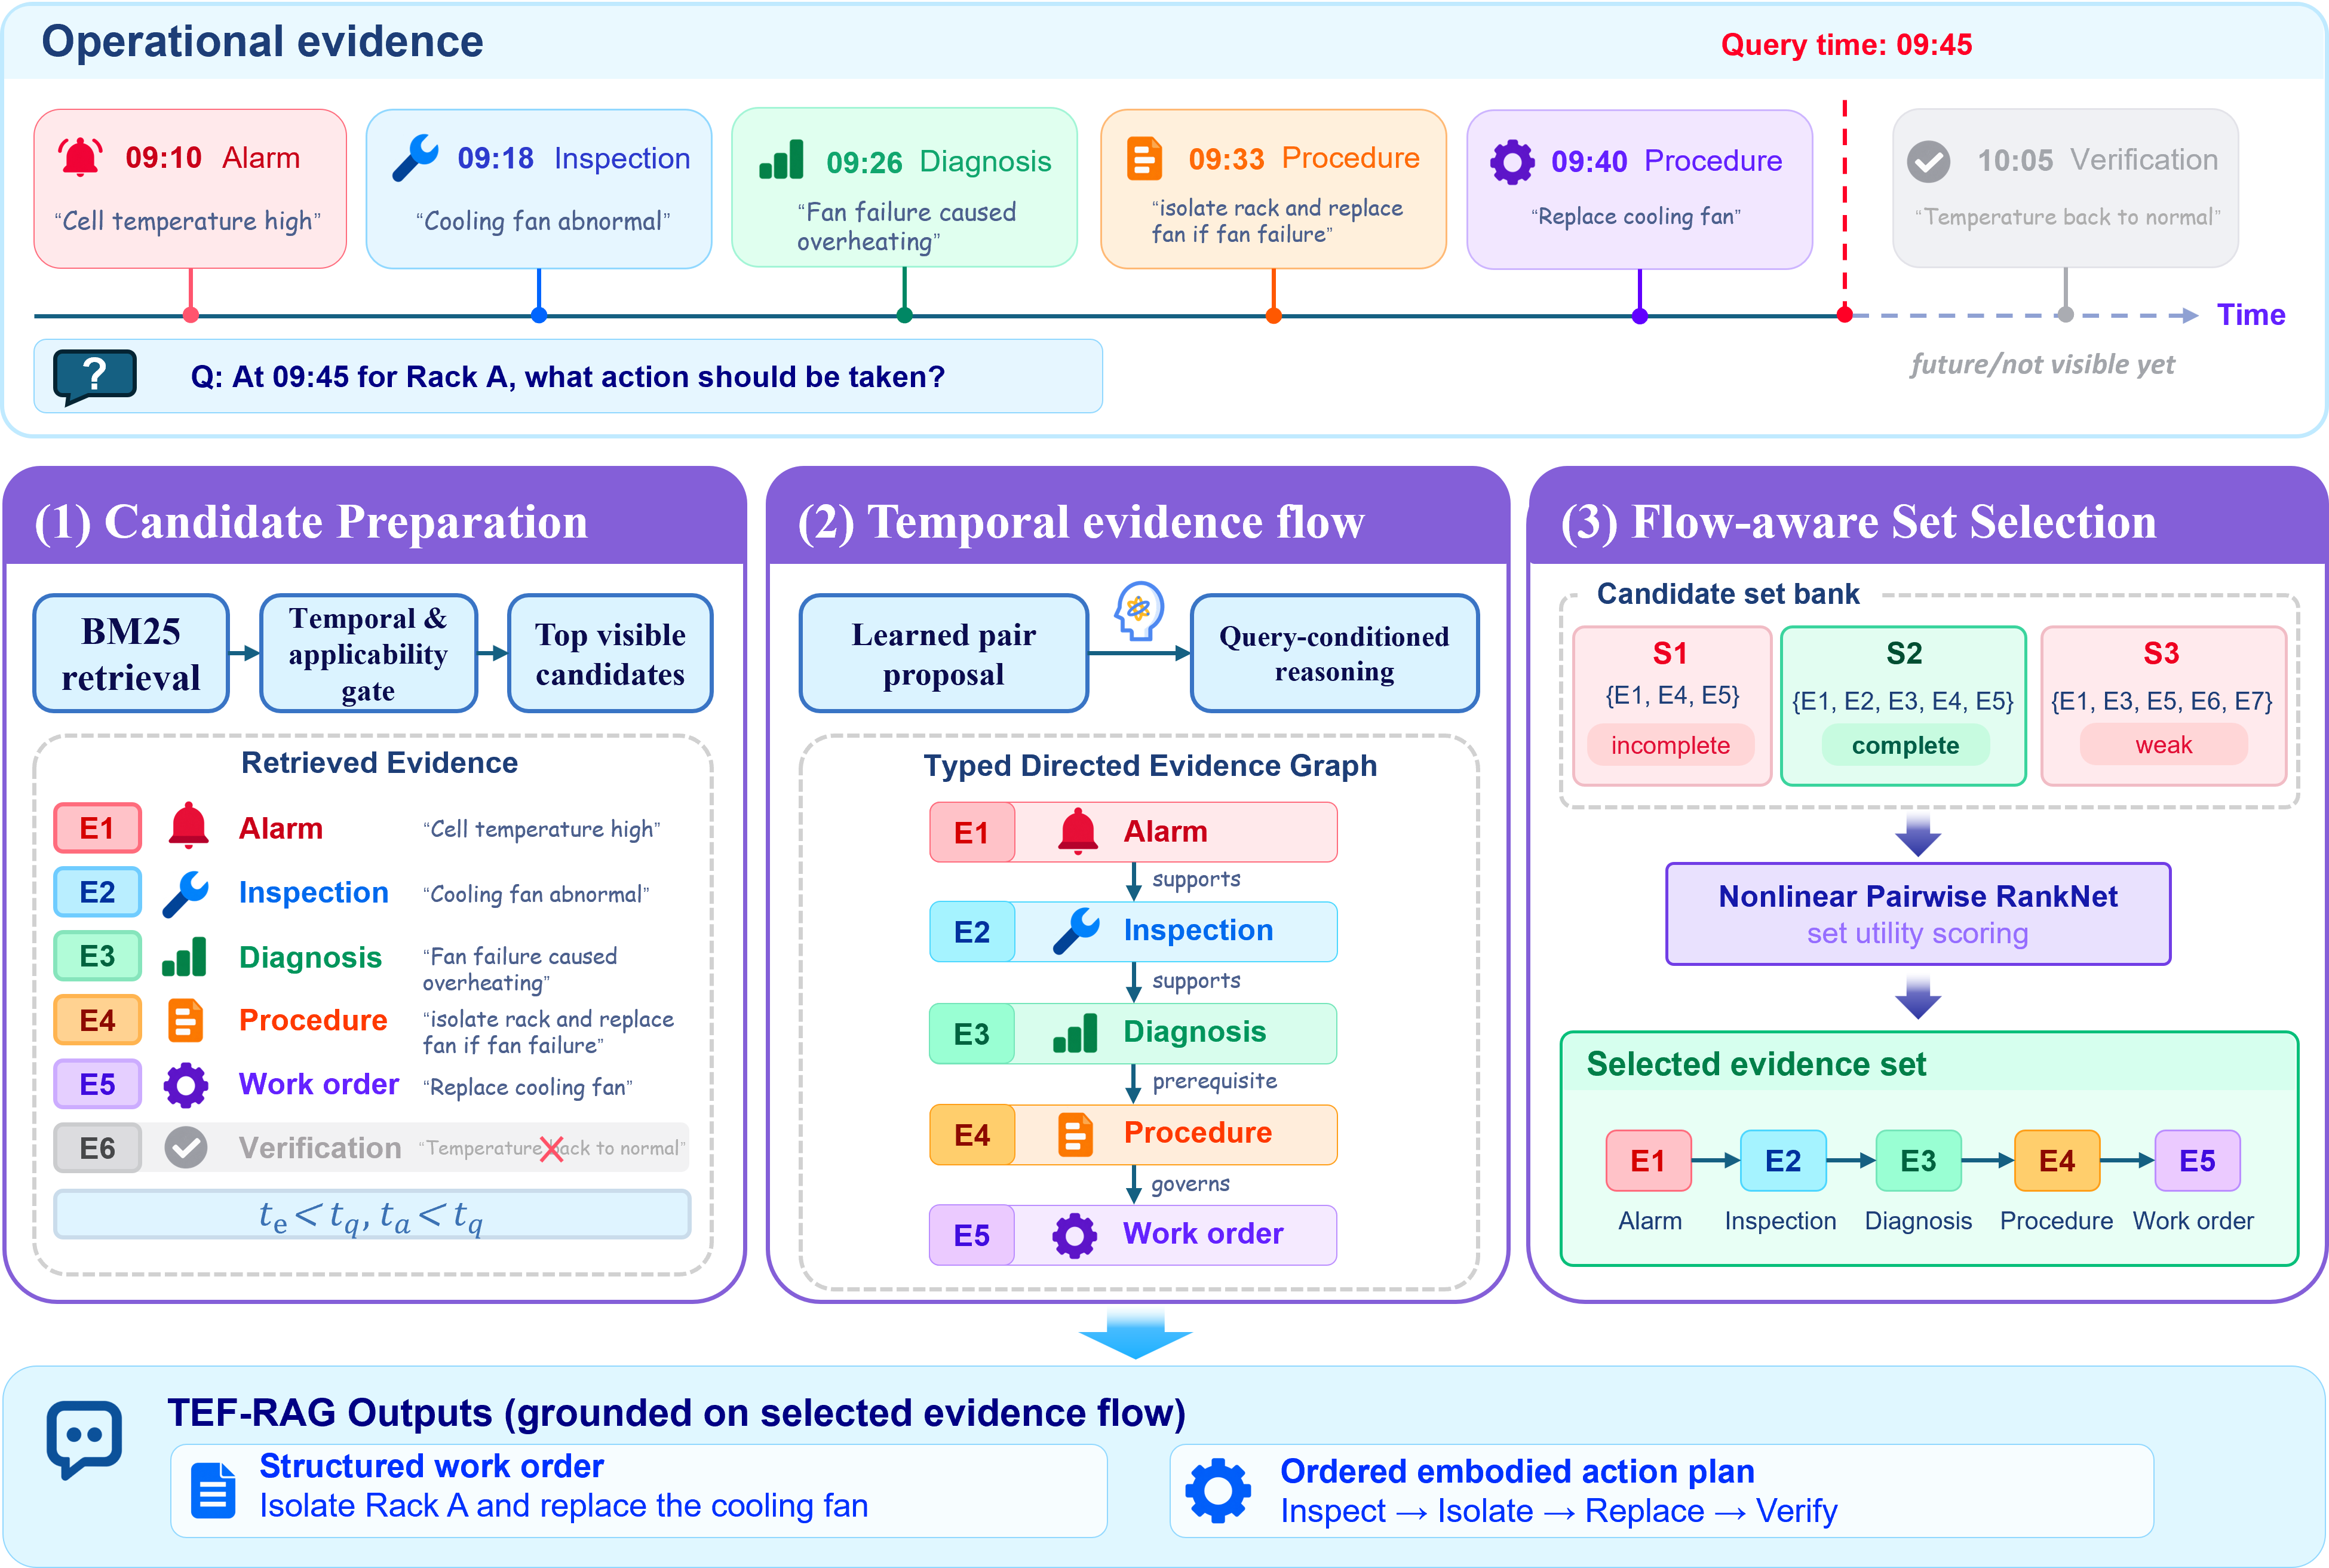
\includegraphics[width=0.96\textwidth]{figures/tef_rag_overview.png}
    \caption{Overview of TEF-RAG. The system first selects candidate evidence pairs from records that are legal at the query time, then constructs a query-conditioned Temporal Evidence Flow. A nonlinear pairwise ranker selects at most five records from the candidate-set space as the evidence flow, which is then used as controlled context for a shared downstream generator.}
    \label{fig:tef_overview}
\end{figure*}

\subsection{Candidate Evidence Preparation and Temporal Legality}

TEF-RAG first applies a unified legality check to heterogeneous raw records. Records are directly excluded if they refer to the wrong asset, describe events after the query time, become available only after the query time, or correspond to procedures that are inapplicable to the current model or time period. This stage does not learn relevance; instead, it establishes a knowledge boundary that subsequent models cannot override.

Within the legal set $\Candidates_q$, BM25 produces a broad candidate pool. A Top-30 search pool is then formed using features available at retrieval time, including lexical relevance, temporal recency, and compatibility with the roles required by the query. This pool is intended to preserve recall rather than determine the final output directly. If fewer than five legal candidates exist, the system keeps the shorter output without artificial padding.

\subsection{Learned Pair Proposal}

Applying semantic relation reasoning to every ordered pair in the search pool would incur quadratic cost in the number of candidates. TEF-RAG therefore first learns a lightweight pair proposer that estimates, for each temporally valid evidence pair $(e_i,e_j)$, the probability that the pair is worth passing to the relation-reasoning stage:
\begin{equation}
p_{ij}
=
\sigma\!\left(
\mathbf{w}^{\top}\phi_p(q,e_i,e_j)+b
\right).
\label{eq:pair_proposal}
\end{equation}

Here, $\phi_p(q,e_i,e_j)$ denotes the feature representation of query $q$ and evidence pair $(e_i,e_j)$. It includes textual relevance between the query and both records, similarity between the two records, event types, temporal gaps, and supersession-related information. If an evidence pair realizes a required relation in an annotated reference evidence flow from the training data, it is treated as a positive sample; all other temporally valid pairs are treated as negative samples. Logistic regression is then used to learn the priority of each candidate pair, and only high-scoring pairs are forwarded to the subsequent relation-reasoning module.

The primary purpose of pair proposal is therefore to focus a fixed semantic-reasoning budget on more promising evidence pairs while preserving the deterministic temporal direction constraint.

\subsection{Query-Conditioned Temporal Evidence Flow}

For each retained candidate pair, TEF-RAG uses a query-conditioned LLM relation judge that reads the query together with the text and metadata of both evidence records and outputs
\begin{equation}
h_{\eta}(q,e_i,e_j)
\rightarrow
(r_{ij},c_{ij}),
\end{equation}
where $r_{ij}\in\Rels$ and $c_{ij}\in[0,1]$ is the relation confidence. Only pairs predicted to have a valid relation and exceeding the confidence threshold are added to the graph. If no sufficiently clear semantic relation is identified, the pair is discarded. The fixed prompt used by the relation judge is provided in Appendix~\ref{app:relation_prompt}.

Candidate evidence records are treated as graph nodes, and identified semantic relations between two records are represented as directed edges. For query $q$, the Temporal Evidence Flow graph is
\begin{equation}
\FlowGraph_q=(V_q,E_q),
\end{equation}
where $V_q$ is the candidate evidence set and $E_q$ is the set of evidence relations. Each directed relation edge can be written as $(e_i,r,e_j)$, meaning that evidence $e_i$ points to evidence $e_j$ through relation $r$, where $r\in\Rels$.

The relation vocabulary includes process-oriented relations such as supports, governs, qualifies, contrasts, prerequisite, preserves uncertainty, resolves, supersession, updates, and verifies. Edge direction follows event time or an explicit prerequisite/update direction, allowing the graph to branch and merge rather than forcing it into a single path.

Unlike a static knowledge graph, $\FlowGraph_q$ is query-conditioned: the same pair of records may play different task roles under different queries. The relation judge also cannot override the legality boundary defined in Section~\ref{sec:problem}; thus, late-arriving evidence, future events, and inapplicable procedures cannot re-enter the candidate set through semantic reasoning.

\subsection{Candidate Evidence-Set Construction}

After the relation graph is built, TEF-RAG compares different evidence combinations rather than continuing to rank individual records independently. Enumerating all five-record combinations from the full search pool is expensive, so we construct only a collection of promising candidate sets.

Specifically, we enumerate five-record combinations from the highest-scoring evidence nodes to cover different combinations of highly relevant records. We also retain high-quality sets produced by earlier search stages and perform single-record replacements around these sets, allowing lower-ranked evidence that fills a critical task role to enter the candidate bank.

For each set $\Selected$, we extract a set-level representation $\phi_s(q,\Selected,\FlowGraph_q)$. The final model uses 62 features covering:
\begin{itemize}
    \item statistics of node relevance, temporal scores, and role compatibility;
    \item coverage of event types and source types;
    \item the number of valid internal edges, edge confidence, connected components, and the longest directed path;
    \item temporal span, average event gap, and source/text diversity;
    \item penalty signals for redundancy, missing roles, and isolated nodes.
\end{itemize}
Together, these features describe whether the selected evidence forms a complete task-support structure as a whole rather than merely repeating individual node scores.

\subsection{Nonlinear Pairwise Set Ranking}

The final ranker is a small nonlinear RankNet~\cite{burges2005ranknet}. Let
\begin{equation}
s_{\theta}(q,\Selected)
=
\operatorname{MLP}_{\theta}
\!\left(
\phi_s(q,\Selected,\FlowGraph_q)
\right).
\end{equation}
The final stage uses pairwise preference learning over evidence sets. For the same query, the candidate bank typically contains multiple complete sets and multiple incomplete sets. We construct training pairs
$(\Selected_i^+,\Selected_j^-)$,
where $\Selected_i^+$ is a candidate set that can form a complete reference evidence flow and $\Selected_j^-$ is a candidate set that misses critical evidence or contains an incomplete relation structure.

For each training pair, the ranker is trained to assign a higher score to the complete set:
\begin{equation}
\ell(q,\Selected_i^+,\Selected_j^-)
=
-\log \sigma\left(
s_{\theta}(q,\Selected_i^+)
-
s_{\theta}(q,\Selected_j^-)
\right).
\label{eq:ranknet_pair_loss}
\end{equation}

The final objective averages the loss across all training pairs:
\begin{equation}
\mathcal{L}
=
\frac{1}{|\mathcal{P}|}
\sum_{(q,\Selected_i^+,\Selected_j^-)\in\mathcal{P}}
\ell(q,\Selected_i^+,\Selected_j^-),
\label{eq:ranknet_loss}
\end{equation}
where $\mathcal{P}$ denotes all candidate-set pairs constructed during training.

In the first training round, negative samples are prioritized using a rule-based set score. This score combines individual evidence quality, internal set relations, task-role coverage, content redundancy, and isolated evidence; its complete definition is given in Appendix~\ref{app:hand_score}. These sets often contain several highly relevant records but still miss critical evidence or relations, making them harder to distinguish than random negatives. A small number of compositionally diverse negative sets are also retained to increase training diversity.

After the first training round, the current ranker rescoring is applied to all negative sets, and the highest-scoring failed sets are selected as hard negatives. Although these sets are known not to form a complete reference evidence flow, the current model is most likely to rank them near the top. A second training round with these hard negatives further teaches the ranker to distinguish complete from incomplete evidence sets.

\subsection{Interface to the Embodied O\&M Generator}

The output of TEF-RAG is not a low-level robotic control command, but an evidence context for downstream embodied execution. A shared downstream generator takes the query and retrieved evidence to produce a standardized work order and a dependency-aware action plan; these structured outputs can then be passed to a planner, constraint checker, or robotic executor.

To isolate the effect of retrieval quality, all compared methods share the same downstream generator. The generator receives only the query and the evidence records selected by the current retrieval method; it does not receive the method name, retrieval scores, or TEF graph structure. The fixed generation prompt is provided in Appendix~\ref{app:generation_prompt}. Our evaluation stops at the structured work order and action plan, and does not treat closed-loop robotic execution or field safety certification as solved problems.
